\documentclass[12pt,a4paper,oneside]{NITR}

\usepackage[hyphens]{url} 
%\usepackage[usenames,dvipsnames]{color}
%\usepackage[colorlinks=true,breaklinks,backref=true,linkcolor={MidnightBlue},citecolor={Fuchsia},urlcolor={OliveGreen}]{hyperref}
\usepackage[none]{hyphenat}
\usepackage{amsmath,amsfonts,mathdots,amssymb,yfonts}
\usepackage{graphicx}
\usepackage{tikz}
\usetikzlibrary{trees,shapes}
\usepackage{booktabs}
\usepackage{algorithm}
\usepackage{algorithmic}
\usepackage{float}
%\usepackage{subfigure}
%\usepackage[ruled,linesnumbered,slide,vlined]{algorithm2e}
%\usepackage{verbatim}
%\usepackage{wrapfig}
%\usepackage{multirow}
%% % % % % % %
\onehalfspacing
\begin{document}
\sloppy
% % % % % % % % % % % % % % % % % % % % % % % % % % %
% % % % % % % % % % % % % % % % % % % % % % % % % % %
\author{Koshal Kumar Garg}
\rollNumber{114CS0100}
\authorGender{male}		%%Author's gender: male or female
\department{Department of Computer Science and Engineering}
\docTitle{Anomaly Detection in Streaming Data}

% % % % % % % % % % % % % % % % % % % % % % % % % % % % % %
% % % % % % % % % % % % % % % % % % % % % % % % % % % % % %
% % % Use any ONE of the following three as appropriate

%%\studentType{doctoral}			
%%\studentType{postgraduate}	
\studentType{undergraduate}
	
% % % % % % % % % % % % % % % % % % % % % % % % % % % % % %
% % % Use any ONE of the following as appropriate

%%\degree{Doctor of Philosophy} 				 %%Doctor of Philosophy; 
%%\degree{Master of Arts}					 %%Master of Arts;
%%\degree{Master of Technology}				 %%Master of Technology;
\degree{Bachelor of Technology}			 %%Bachelor of Technology;
%%\degree{Master of Business Administration} %%Master of Business Administration;

% % % % % % % % % % % % % % % % % % % % % % % % % % % % % %
% % % % % % % % % % % % % % % % % % % % % % % % % % % % % %

% % % Mention the discipline in which the degree is awarded
\degreeIn{Computer Science and Engineering}		

% % % Mention the specialization with which the degree is awarded. 
% %\specialization{Information Security}	

% % % % % % % % % % % % % % % % % % % % % % % % % % % % % %
% % % % % % % % % % % % % % % % % % % % % % % % % % % % % %

\docType{2}		%%Dissertation=1; Thesis=2; Project=3; Synopsis=4; Registration Report=5

% % % % % % % % % % % % % % % % % % % % % % % % % % % % % %
% % % % % % % % % % % % % % % % % % % % % % % % % % % % % %

\numOfSupervisors{1}

\principalSupervisor{Bidyut Kumar Patra}	%%Name only
%%\coSupervisor{Homi Jehangir Bhabha}			%%Name only
%%\firstMemberDSC{Carl Friedrich Gauss}		%%Name only
%%\secondMemberDSC{Isaac Newton}				%%Name only
%%\thirdMemberDSC{Dennis Ritchie}				%%Name only
%%\externalExaminer{Niels Bohr}				%%Name only
%%\chairperson{Aryabhata}						%%Name only
%%\hod{Varahamihira}							%%Name only

\principalSupervisorDesignation{Associate Professor}
%%\coSupervisorDesignation{Associate Professor}

% % % % % % % % % % % % % % % % % % % % % % % % % % % % % %
% % % % % % % % % % % % % % % % % % % % % % % % % % % % % %

\setDate{14}
\setMonth{May}
\setYear{2018}

% % % % % % % % % % % % % % % % % % % % % % % % % % % % % %
% % % % % % % % % % % % % % % % % % % % % % % % % % % % % %

\Font{1}	%% Times New Roman=1; Arial=2;
\setFont

% % % % % % % % % % % % % % % % % % % % % % % % % % % % % %
% % % % % % % % % % % % % % % % % % % % % % % % % % % % % %
% % % These may be used to fine tune the cover and title pages

\titlePageLineSpacing{2}
\titleWidth{.75}
\titleCoordinateX{0.16}
\titleCoordinateY{0.12}

% % % % % % % % % % % % % % % % % % % % % % % % % % %
% % % % % % % % % % % % % % % % % % % % % % % % % % %
% % % % % % % % % % % % % % % % % % % % % % % % % % %
	% %Fill details in "FrontPages.tex"
% % % % % % % % % % % % % % % % % % % % % % % % % % %
% % % % % % % % % % % % % % % % % % % % % % % % % % %
%%\coverPageSynReg		% %Needed for Synopsis Cover Page or 
						% %Registration Report Cover Page.
						% %To be used along with "\docType()".
						% %Use "\section{Introduction}\label{Guidelines}
Submission of synopsis or extended abstract is one of the mandatory requirements before submitting a doctoral or master thesis. It is not just a longer version of an abstract. It is as good as a research paper that conveys the essence of the thesis without overlooking the importance of introduction and conclusion. A synopsis should include the following~\textemdash~
\begin{itemize}
	\item Introduction
	\item Aim
	\item Method
	\item Results
	\item Conclusion
	\item Limitations
	\item References
	\item Dissemination
\end{itemize}

\noindent A synopsis is a self-contained, capsule description of the thesis that must make sense all by itself. Typical length of a synopsis should be between 5 and 10. Pages must of A4 dimension with 25mm margin on all four sides. The entire dissertation must be written using only a single font including all the texts inside graphs, figures, block diagrams, etc. While writing captions of tables and figures, the font size should be decreased by one point. Similarly, the font size of bibliography and index should also be lessened by a point. Students are advised to use the following in the body text~\textemdash
\begin{itemize}
\item[] serif fonts like Times New Roman (TNR) of size 12pt \\
or \\
\textsf{sans-serif fonts like Arial of size 11pt}. 
\end{itemize}
Needless to say that the use of font should be uniform throughout. Headings, Titles \textit{etc.} should use fonts as given below in Table~\ref{tab-fonts}.
{
\linespread{1}
\begin{table}[h]
\centering
\caption{Font sizes to be used in the dissertation}
\begin{tabular}{l C{25mm} C{25mm} c} 
\toprule
{Item} & Arial & {TNR} & {Justification}\\
\midrule\midrule
Main Text & 11 normal & 12 normal & Justified \\
\midrule
Sub-sub Heading & 11 bold & 12 bold & Left \\
\midrule
Sub Heading & 13 bold & 14 bold & Left \\
\midrule
Heading$^{\#}$ & 16 bold & 17 bold & Left \\
\midrule
Chapter Title & 22 bold & 24 bold & Center \\
\midrule
Chapter Number & 16 bold & 17 bold & Left \\
\bottomrule
\multicolumn{4}{l}{$^{\#}$Add serial number with one decimal place.} 
\end{tabular}
\label{tab-fonts}
\end{table}
}
\par The class file \texttt{NITR.cls} can be used to prepare a synopsis. One needs to invoke the statement ``\texttt{\textbackslash synopsisCoverPage}'' in the main ``\texttt{.tex}'' file with ``\texttt{\textbackslash docType(4)}'' and all necessary data in the ``\texttt{FrontPages.tex}''. The text of the synopsis can be written in ``\texttt{./SynopsisText/SynopsisText.tex}''."
						% %Comment rest.
\coverPage
\titlePage
%%\certificateOfExamination

\certificateOneSupervisor		%% Comment any
%%\certificateTwoSupervisors		%% one of these two

%\dedication
\declaration
\acknowledgment
\abstract
% % % % % % % % % % % % % % % % % % % % % % % % % % %
% % % % % % % % % % % % % % % % % % % % % % % % % % %
\tableofcontents
\cleardoublepage
% % % % % % % % % % % % % % % % % % % % % % % % % % %
% % % % % % % % % % % % % % % % % % % % % % % % % % %
\addcontentsline{toc}{chapter}{List of Figures}
\listoffigures
\cleardoublepage
% % % % % % % % % % % % % % % % %
\addcontentsline{toc}{chapter}{List of Tables}
\listoftables
\cleardoublepage
% % % % % % % % % % % % % % % % % % % % % % % % % % %
% % % % % % % % % % % % % % % % % % % % % % % % % % %
\pagenumbering{arabic}
\pagestyle{fancy}
\renewcommand{\chaptermark}[1]{\markboth{#1}{}}
\renewcommand{\sectionmark}[1]{\markright{\textbf{Chapter \thechapter}}}
% % % % % % % % % % % % % % % % % % % % % % % % % % %
% % % % % % % % % % % % % % % % % % % % % % % % % % %
%Formatting Guidelines for Writing Dissertation.
\chapter{Introduction}

We are living in a world where data plays a vital role in daily life as well as in the
business and different organization. Thus, the efficient analysis of the data is vital.
However, there may be some data points in a dataset which may diminish the quality
of the analysis done or which may be of some special interest to the user. Such
points are referred to as Outliers. Outliers are the points which deviate significantly from rest of the data. They do not conform to an expected pattern. The importance of anomaly detection is due to the fact that anomalies in data translate
to significant, and often critical, actionable information in a wide variety of application
domains. Sometimes in applications like sensor networks the anomalies has to be found out on fly dynamically. The results are expected instantaneously. Hence Outlier detection techniques have to be computationally fast enough to address huge amount of data generated continuously in data streams.  Hawkins
\cite{hawkins} defined the outlier as:

\par 
\textit{An outlier is an observation that deviates so much from other observations as to
	arouse suspicion that it was generated by a different mechanism.}
 
	 However, outlier detection on streaming data is particularly
challenging, since the volume of data to be analyzed is
effectively unbounded and cannot be stored indefinitely in
memory for processing \cite{c}. Data streams are generated at a high data rate and hence the computation speed and efficiency of algorithm has to be high. An outlier detection system in wireless sensor
networks must work with the limited memory in each
sensor node in order to detect rare events in near real time. In the
case of data streams, where the number of data points is
unbounded and can arrive at a high rate, keeping all data
points is impossible. Simply deleting some of the points does not help because it may affect the accuracy and detection efficiency of upcoming points. Deleting previous points can cause two problems: i) Deleting the previous data points decreases the detection accuracy of local outlier factor for new data points, ii)We can not differentiate between past events and new events. 


Anomaly detection refers to the problem of finding patterns in data that do not conform
to expected behavior. These nonconforming patterns are often referred to as anomalies,
outliers, discordant observations, exceptions, aberrations, surprises, peculiarities, or contaminants in different application domains \cite{a}. Anomalies are patterns in data that do not conform to a well defined notion of normal
behavior.

\section{Overview}

Some of the prerequisites that is essential for the study of anomaly detection are described in this section. Depending on different domains and data types, approach of anomaly detection varies. 
\subsection{Aspects of Anomaly Detection}

\begin{enumerate}
	\item \textit{Nature of Input Data} : Input
	is generally a collection of data instances. Each data instance contains some attribute values. Attributes can be of different type such as binary, categorical, or continuous. For nearest-neighbor-based techniques, the pairwise distance between instances might be
	provided in the form of a distance or similarity matrix. In such cases, techniques that
	require original data instances are not applicable.
	
	\item \textit{Type of Anomaly} :  
	Anomalies are of three types
	\begin{enumerate}
		\item \textit{Point Anomalies} : If a single data instance is considerd outlier to rest of the data points then it is called point anomaly. For examle in credit card  fraud detection the data instance the amount spent is very high compared to the normal range of expenditure
		for that person will be a point anomaly.
		
		\item \textit{Contextual Anomalies} : If a data point is considered anomaly in certain context but not otherwise then it  is called contextual or conditional anomaly \cite{contextual}. For example 1000 dollar expense per week may be considered anomaly in a normal week but not in Christmas week.
		
		\item \textit{Collective Anomalies} : If a collection of related data points are anomalous with respect to entire data set then they are termed as collective anomalies. Individually these data points may not be anomalous but taking together they are outliers. Collective outliers are mainly explored for sequence data \cite{ca1},
		graph data \cite{ca2} and spatial data \cite{ca3}.
	\end{enumerate}
	
	
	
	\item \textit{Data Labels} : 
	Data labels for each instance shows whether it is a normal point or anomalous. Labeling is often done manually by a human expert which is clearly very expensive and time taking. Getting a training data set that contains the representative of all possible outliers is very difficult. Based on the extend of availability of labeled data, anomaly detection technique can operate in three modes
	
	\begin{enumerate}
		
		\item \textit{Supervised Anomaly Detection} : Training data set that has labeled instances for both normal and anomalous class. Any new data instances is classified in one among these two classes. Major problem with this approach is to get labeled data and anomalous instances are very few as compared to normal instances. This imbalanced class distribution reduces the accuracy. 
		
		\item \textit{Semisupervised Anomaly Detection.} : Training data set has labeled instances for either normal or anomalous class only. It is very difficult to put representative instances for all possible outliers that can occur in the data.
		
		\item \textit{Unsupervised Anomaly Detection} : In unsupervised anomaly detection there is no training data. This works with the assumption that normal instances are far more than anomalies in test data.   
	\end{enumerate}
	
	
	\item \textit{Output of Anomaly Detection}
	
	\begin{enumerate}
		\item \textit{Scores} : Score is assigned to each instance depending on the degree to which that instance is considered anomaly. Selecting the cutoff for anomaly is decided based on the number of top anomalous points.
		
		\item \textit{Label} : Binary label is assigned to each instance whether it is normal or anomalous.
	\end{enumerate} 
	
	
\end{enumerate}

\subsection{Common Causes of Outlier on a Dataset}





\begin{itemize}
	\item Data entry errors : These errors are introduced artificially by the humans while
	collecting the data or while recording the data. These errors may result into an
	outlier in th data set.
	
	
	\item Measurment errors : This error occurs artificially while measuring the reading of
	the data set. This can occur due to a faulty machine or due to human error. For eg- While testing the blood sample of any patient, the machine can give false
	reading for the sugar level test which will be declared as an outlier.
	
	\item Data processing errors : During the data analysis, the data in pre-processed
	and many manipulation is being made. While doing so, outliers can be accidently
	introduced to the data set or the changes made to particular data point can also
	result in outliers.
	\item Sampling errors : Extracting or mixing data from wrong or various sources
	
	\item Natural : Those that are not a product of an error are called novelties.
	
\end{itemize} 



\subsection{Anomaly Detection Techniques} 

\begin{enumerate}
	\item \textit {Nearest Neighbor Based } : Nearest neighbor based anomaly detection techniques works on the assumption that normal data points occur in dense clusters and oultliers lie far from their neighbors. It requires a distance or similarity
	measure defined between two data instances. Nearest neighbor based technique is broadly classified in two types
	
	\begin{enumerate}
		\item 
		\textit{Using Distance to $K^{th}$  Nearest Neighbor}
		The anomaly score of an instance is the distance between the point and it's $K^{th}$ nearest neighbor. A different approach to compute anomaly score is to count no of instances in a radius of d. 
		
		\item 
		\textit{Using Relative Density} : An instance that lies in a neighborhood of less density is considered outlier while an instance that lies in a dense neighborhood is considered normal. But this technique fails for dataset with varying densities. To address this problem the density of instances relative to their neighborhood is computed.
		
		\par To assign a relative density score, Local Outlier Factor was proposed. For any given data instance, the LOF score is equal to
		ratio of average local density of the k nearest neighbors of the instance and the local
		density of the data instance itself \cite{b}.
		
	\end{enumerate}
	
	
	
	\item \textit{Clustering Based Anomaly Detection Techniques} : 
	
	Clustering is grouping similar data points into clusters. Clustering is unsupervised. These techniques work on the assumption that
	\begin{itemize}
		\item Normal points lie inside clusters and anomalous points does not belong to any cluster.
		
		\item Normal points lie closer to the cluster center while outliers lie far away from the cluster centers.
		
		\item Normal data points belongs to large and dense clusters while outliers belong to small and parse clusters.
	\end{itemize} 
	
	
	
\end{enumerate}

\subsection{Applications of Anomaly Detection}


\begin{enumerate}
	
\item \textbf{Intrusion Detection}\
Intrusion detection refers to detection of malicious activity in a computer related system. An intrusion is different from normal behavior of computer and hence anomaly detection techniques are applicable for intrusion detection domain. The main challenges for this domain are huge amount of data and streaming data. Anomaly detection has to be performed online. Moreover due to huge data, there is possibility of false alarm. Hence for this domain supervised anomaly detection techniques are preferable because they can have labeled data for normal behavior. 
	 

\item \textbf{Fraud Detection}\

Fraud detection refers to detection of criminal activities occurring in commercial organizations
such as banks, credit card companies, insurance agencies, cell phone companies,
stock market, and so on. If the user is not actual customer of the organization then it is called identity theft. It is considered fraud when user tries to access resources of the organization without any authorization. It is necessary to recognize these fraud activities immediately to prevent economic losses. Clustering \cite{fraud} is the
unsupervised method used for the fraud detection.


\item \textbf{Medical and Public Health Anomaly Detection}\

In this domain anomalies are to be found in patient records. Anomalies may occur due to various reasons such as abnormal
patient condition, instrumentation errors, or recording errors. Patient data consists of several different types of features,
such as patient age, blood group, and weight. Most of the current anomaly detection techniques in this
domain aim at detecting anomalous records, point anomalies. Typically the labeled
data belongs to the healthy patients, hence most of the techniques adopt a semi supervised
approach \cite{medical} . 


\item \textbf{Industrial Damage Detection}\

The data in this domain are mostly sensor data. Industrial damage detection
can be classified into two domains, one that deals with defects in mechanical
components such as motors, engines, and so on, and the other that deals with defects
in physical structures. The former domain is also referred to as system health
management.


\item \textbf{Traffic Anomaly Detection}\

In this  domain 
anomalous behavior of vehicles due to the traffic congestion are detected. Based on the regular trajectories of the taxi cabs, if the trajectory on a certain differs then it is considered as outlier. This change in behavior is due to the heavy traffic in the regular trajectory. Detection of such anomalies can save a lot of time and fuel.   

\end{enumerate}



 
	
\section{Motivation}
Outlier detection has many applications and hence its study to improvise its accuracy and decrease the computation time is the objective of this research. Many static anomaly detection techniques like Local Outlier Factor have been proposed but now a days data that has to be analyzed are not static. Data is generated continuously in data streams and detection of anomaly in data streams is quite challenging. 

\par

We need an incremental outlier detection technique that can work online and detect outliers as soon as they enter dataset. One of the incremental approach is Incremental LOF(iLOF). But this approach is not practical because it stores all the data points that has ever be analyzed. We have limited memory to store only some of the data points. So the motivation of this research project is to find an outlier detection technique which is incremental as well as memory efficient.  

	
	
	
\section{Contribution of the Thesis}
In order to achieve the objective of this project, we have used Local Outlier Factor as the anomaly score to find out anomalies in datasets and then compare these results with different incremental outlier detection techniques. 

\par
In incremental approaches, we don't have enough memory to store all the data points. Gradually the size will increase and hence the computation time. In order to do it in a memory efficient way we have to delete some of the data points and summarize them. But the selection of the points that has to be deleted need to be done carefully because these points may have vital information for the upcoming data points. We propose a memory efficient incremental outlier detection technique which is an extension to Memory efficient Incremental LOF(MiLOF) which uses Reverse $K$ Nearest Neighbors(RKNN) counts for all the data points.

\section{Thesis Organization}

The thesis is organized as follows.

\begin{itemize}
	
\item  \textbf{Chapter 2 :} This chapter includes the summary of different approaches which are available for anomaly detection.

\item  \textbf{Chapter 3 :} This chapter describes the contribution of the thesis. In this chapter we have explained our proposed work and compared the results with previous approaches.



\item \textbf{Chapter 4 :} This chapter summarizes overall contributions and discusses a future research
directions of the thesis.

 


\end{itemize}
	





\thispagestyle{empty}
\cleardoublepage
% % % % % % % % % % % % % % % % % % % % % % % % % % %
% % % % % % % % % % % % % % % % % % % % % % % % % % %
%Some Unstructured Advice on Dissertation Writing
\chapter{Literature Survey}\label{Unstructured}


%Outside the domain of physical formatting and layout, this document does not intend to foray into the contents of the dissertation to be written. That would influence contents and stubble creativity. The following unstructured guidelines, however, may sometime prove useful to the students and their guides, who are looking for a good model.



	
	\section{LOF: Identifying Density-Based Local Outliers}
	Local Outlier Factor is a score assigned to each of the data points based on the degree on how
	isolated the object is with respect to the surrounding neighborhood \cite{b}.
	The outlier factor is local
	in the sense that only a restricted neighborhood of each object is taken into account.We show that
	for most objects in a cluster their LOF are approximately equal to 1. Following are the terms which are used to compute LOF of a data point.
	
	
		\begin{itemize}
		\item \textbf{K-distance} :The distance between a data point p
		and its $K^{th}$ nearest neighbor (K-NN).
		
		\item \textbf{Reachability distance (reach-dist)} of a data point p
		with respect to another data point o
		
		\[ reach-dist_K(p,o)=max\{k-distance(o),d(p,o)\}  \]
		
		where d(p,o) is the euclidean distance between p
		and o.
		
		
		\item \textbf{Local Reachability Density(lrd)}  of a data point p
		
		
		\[  lrd_k(p) =  \bigg( \frac{1}{K} \sum_{o \in N_{(p,k)}} reach-dist(p,o)   \bigg)^{-1}  \]
		
		
		where $N_{(p,k)}$ is the set of k nearest neighbors of p.
		
		\item
		\textbf{Local Outlier Factor(LOF)}  of a data point p
		
		\[  LOF_K(p) = \frac{1}{K} \sum_{o \in N_{(p,k)}} \frac{lrd_K(o)}{lrd_K(p)}  \]
		
	\end{itemize}
	
		\begin{figure}[H]
		\centering
		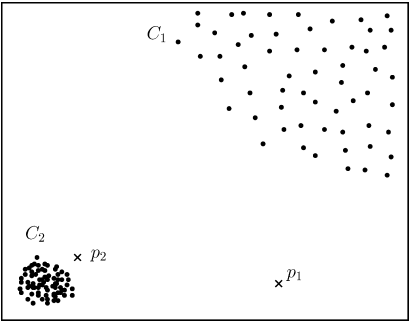
\includegraphics{chap01/localvsglobal.png}
		\caption{Limitations of Global outlier detection}
	\end{figure}
	
	
	
	\par 
	Local density based outlier detection is preferred over global because global density based techniques performs poorly for datasets with varying densities.
	Consider the 2-D data set shown in Figure 2.1, both points p1 and p2 should be detected as outliers. But if we consider global density, p2 will not be detected as outlier because of low density of cluster C1. For a point q in cluster C1, the distance between q and its nearest neighbor will always be greater than distance between p2 and its nearest neighbor.
	


	
	
	\section{Incremental Local Outlier Detection for Data Streams}
	Incremental LOF for data streams refer to computation LOF score of newly added data points and updating the same for older data points. Outlier detection techniques are categorized into 4 types \cite{f}
	
	\begin{enumerate}
		\item \textit{Statistical Approach} : the data points are typically modeled using a stochastic distribution, and points are labeled as outliers depending on their relationship with this model.
		
		\item \textit{Distance Based Approach} : detect outliers by computing distances among points.
		
		\item \textit{Profiling Methods} : Profiles of normal behavior is built and deviation from that are considered outliers.
		
		\item \textit{Model-based Approach} : First characterization of normal points using predictive models like neural networks and SVM. Deviation from these models are considered outliers.
		
		
	\end{enumerate}
	
	Static LOF algorithms can be applied to data stream is three ways. However these are computationally inefficient.
	
	\begin{enumerate}
		\item \textit{Periodic LOF} : Static LOF is applied periodically on entire data set every time new data blocks are entered. The problem with such approach is that a data point which may be anomalous while added may not be detected as outlier later as many other points are added. they may create a cluster of their own and outliers will be missed. If LOF is computed each time a data point is added, the change is behavior can be detected at that moment.
		
		\item \textit{Supervised LOF} : K-distance, lrd and LOF of the data points are precomputed. Any new data point that arrives all these parameters are computed without updating for previous points. As a result the LOF accuracy decreases. 
		
		\item \textit{Iterated LOF} : Aplpy static LOF every time a new data point enters. This gives high accuracy at a cost of very high computational time. 
		
		
	\end{enumerate} 
	

	\begin{algorithm}[H]
		\caption{iLOF Insertion}
		\begin{algorithmic}
			\STATE  
			\STATE INPUT:  A data point $p_t$ at time t
			\STATE OUTPUT: LOF value LOF($p_t$)
			\STATE
			
			\STATE Compute KNN and K-distance of $p_t$
			
			\FOR {all o \in KNN($p_t$)}	
			
			\STATE Compute \texttt{reach-dist($p_t$,o)}
			
			\ENDFOR
			
			\STATE  $S_{update}$ \leftarrow Reverse KNNs of $p_t$
			
			\FOR{ all o \in $S_{update}$ and q \in $N_{(o,k)}$}
			
			\STATE Update K-distance(o) and reach-dist(q,o)
			
			\IF {o \in  $N_{(q,k)}$}
			
			\STATE $S_{update}$ \leftarrow  $S_{update}$ \cup q
			\ENDIF
			
			\ENDFOR
			
			\FOR { all o \in $S_{update}$ }
			
			\STATE Update lrd(o) and LOF(R-KNN(o,k))
			
			\ENDFOR
			\STATE Compute lrd($p_t$) and LOF($p_t$)
			\RETURN LOF
			
			
		\end{algorithmic}
	\end{algorithm}

In Incremental approach, LOF score is computed as soon as a data enters. It is determined whether it is outlier or not. LOF of other data points are also updated. 


The algorithm for insertion of a data point in iLOF is given in Algorithm 1. First we compute the K nearest neighbors of new point $p_t$. To update the led and LOf of affected points we compute the reverse K nearest neighbors(RKNN) of these points. All these points are kept in an array called $S_update$. Finally for all these points, lrd and LOF value is computed.  

	

\section{Dolphin}

Dolphin is a distance based outlier detection technique for disk resident datasets. The algorithm receives
as input a disk-resident dataset DS and parameters k and R, and outputs all
and only the DB(k,R) outliers of DS. Dolphin does two scans to find all the outlier points \cite{e}.

\subsection{Algorithm}

DOLPHIN gains efficiency by naturally merging together in a unified
schema three strategies, namely

\begin{enumerate}
	\item 
	The selection policy of objects to be maintained in main memory
	
	\item Usage of pruning rules
	\item Similarity search techniques
\end{enumerate}


Dolphin uses a part of the main memory and loads a part of the dataset. It maintains a data structure called INDEX while scanning. According to Dolphin , points which do not have at least K points in the radius of R are considered anomalous. Each DBO(Distance Based Outliers) node in INDEX data structure contains

\begin{enumerate}
	\item n.obj : Original Object 
	\item n.id : id of object 
	\item n.nn[h] : an integer array  
\end{enumerate}

n.nn[i] is the number of points which lie at a distance of  \[ \bigg[   {\frac{R}{h}} (i-1) , {\frac{R}{h} } i \bigg] \]  from n.obj.

\[  n.rad = {\frac{R}{h}} i  \ \ \ \           (1 \leq i \leq h) \]
where i i sthe smallest integer such that 

\[  \sum_{j \leq i} n.nn[j]  \ \ \      is \ at \ least \ K-1 \]



After the scan INDEX contains all the outliers but all the points in INDEX need not be outliers. In second scan inliers are removed from INDEX by calling pruneInliers.

\begin{algorithm}[H]
	\caption{Algorithm}
	\begin{algorithmic}
		\STATE  
		\STATE INPUT:  DS Disk Resident Datasets
		\STATE OUTPUT: INDEX containing all the outliers
		\STATE
		
		\STATE Initialize empty INDEX
		
		\FOR {all obj \in DS($p_t$)}	
		
			\STATE $n_{curr}$  $\leftarrow$ obj
			\IF{ ! isInlier( $n_{curr}$ ) }
				\STATE Insert $n_{curr}$ in INDEX
			\ENDIF
		
		\ENDFOR
	
	\STATE  remove from INDEX all the nodes such that n.rad  R
	\STATE  Reset n.nn for all
		
	\end{algorithmic}
\end{algorithm}

In first scan each of the incoming data point, it is decided whether a it is inlier or not by computing distances from the points already in INDEX. If it is not inlier then it is inserted in INDEX. So after first iteration INDEX contains all the outliers. But all the points in INDEX may or may not be outliers. We prune these normal points from INDEX in second scan. In second scan proved inlier are removed and candidate outliers are examined again.  Finally only outliers are present in INDEX.

\begin{algorithm}[H]
	\caption{IsInlier}
	\begin{algorithmic}
		\STATE  
		\STATE INPUT:  $n_{curr}$
		\STATE OUTPUT: Binary (True/Flase)
		\STATE
		
		\STATE Range query search in INDEX
		
		\FOR {all $n_{index}$ \in INDEX}	
		
			\STATE   dst= d($n_{index}$.obj,$n_{curr}$.obj)
			\IF{dst<R-$n_{index}$.rad}
				\RETURN True
			\ENDIF
			
			
			\IF{dst<R}
				\STATE oldRad=$n_{index}$.rad
				\STATE update $n_{index}$.nn[]
				
				\IF{oldRad $>$ R AND $n_{index}$.rad $<$ R}
				 	\STATE  Remove $n_{index}$ from INDEX
				\ENDIF
				
			
			\ENDIF
			
			\STATE  Update $n_{curr}$.nn[]
			
			\IF{$n_{index}$.rad $<$ R}
			   \STATE {$n_{index}$.rad $<$ R} 
			\ENDIF
			
		
		\ENDFOR
		
		\RETURN False
	\end{algorithmic}
\end{algorithm}



\begin{algorithm}[H]
	\caption{PruneInliners}
	\begin{algorithmic}
		\STATE  
		\STATE INPUT: obj
		\STATE
		
		\STATE Range query search in INDEX whith center obj and Radius R
		
		\FOR{ $n_{index}$}
		    \IF {d(bj,$n_{index}$.obj) $<$ R}
	            \STATE Update $n_{index}$.nn[]
 		    \ENDIF
 		    
 		    \IF{$n_{index}$.rad $<$ R}
 		    	\STATE remove $n_{index}$ from INDEX
 		    \ENDIF
		\ENDFOR
		
	\end{algorithmic}
\end{algorithm}


\subsection{Pivoting Based Search Algorithm}

Instead of computing all pairwise distances between points, some pivot points are taken and pairwise distance between all other points are computed. If we have to find distance between two points x and y ,according to triangles inequality

\[  d(x,y) \geq |{d(x,p) - d(y,p)}| \]

\[  d(x,y) \geq D_p(x,y) \]


\[ D(x,y) =MAX_{1 < i <m} D_p(x,y) \]

$D_p(x,y)$ is lower bound of d(x,y). We need to find y such that D(x,y) $<$ R. This returns a superset of y such that d(x,y) $<$ R.





\section{Memory Efficient Incremental Local Outlier Factor (MiLOF)}

Local Outliers detection in data streams when limited memory is available. It is impractical to store all the instances of data streams. Some of the points has to be removed and summarized. Memory available is just sufficient to store K-Distance, lrd and LOF of m data points only.

The available m memory is divided in two parts of size b and c to store original points and summarized points respectively. When memory limit is reached, first ${\frac{b}{2}}$  data points are summarized to c clusters and deleted to free memory \cite{d}. If there already exists summarized data, the old and new cluster centers are merged. Hence at any time maximum memory used is b=m+c.
 Three steps of MiLOF are 

\subsection{Summarization}
Whenever memory reaches limit b, summarization phase is invoked. This phase summarizes first ${\frac{b}{2}}$ points, their K-distance, lrd and LOF and deletes these points from memory. Recent points are retained because data points might have evolved with time and recent points are most important. As the width of the summarization window decreases, it resembles iLOF. So MiLOF is direct generalization of iLOF.

\par 
Summarization  is explained in algorithm 5.
In summarization, if memory is reached first $\frac{b}{2}$ points are summarized to c clusters. K-distance, lrd and LOF for these cluster centers are computed by the following formulas.  

\begin{itemize}
	\item K-Distance of cluster center $v^i_j$ \in $V^i$ 
	
	
		\[  K-Distance(v^i_j) = \frac{\sum_{p \in C^i_j } K-Distance(p)}{| C^i |} \]
		
		
	 \item lrd of cluster center $v^i_j$ \in $V^i$ 
		
		
		\[  lrd_k(v^i_j) = \frac{\sum_{p \in C^i_j } lrd_k(p)}{| C^i |} \]
		
		\item LOF of cluster center $v^i_j$ \in $V^i$ 
		
		
		\[  LOF_k(v^i_j) = \frac{\sum_{p \in C^i_j } LOF_k(p)}{| C^i |} \]
	
\end{itemize}


\begin{algorithm}[h!]
	\caption{MiLOF}
	\begin{algorithmic}
		\STATE  
		\STATE INPUT:  A data point p 
		\STATE OUTPUT: LOF value LOF(p)
		\STATE
		
		\STATE Compute LOF of p 
		\IF {No of points=b}
			\STATE $C^i$ $\leftarrow$ First $\frac{b}{2}$ points
			\STATE ($V^i$,$N^i$) $\leftarrow$ C-means($C^i$)
			
			\FOR {all $v^i$ \in $V^i$} 
			  \STATE Compute avereage K-distance, lrd and LOF
			\ENDFOR
			
			\STATE Delete $C^i$
			
			\IF{i>0}
				\STATE (Z;W) $\leftarrow$ Weighted c-means($V^i$ U $V^{i-1}$ ,$N^i$ U $N^{i-1}$)
				
				\FOR {all z \in Z} 
					\STATE Compute avereage K-distance, lrd and LOF
				\ENDFOR 
				\STATE $V^{i-1}$ \leftarrow Z
				\STATE Delete $V^{i-1}$,Z
				
			\ENDIF	
		\ENDIF
		
		\STATE i $\leftarrow$ i+1
		\RETURN LOF
	\end{algorithmic}
\end{algorithm}

\subsection{Merging}

Summarization is performed every time new $\frac{b}{2}$ new data points arrives. Clustering these points gives c cluster centers $V^i$. These clusters are to be merged with old c cluster centers $V{i-1}$ so that finally only c centers are available. Cluster centers X={$V^i$ U $V^{i-1}$} are merged using a weighted clustering algorithm where weight of each center is no of objects in that cluster. 


\subsection{Revised Insertion}
Whenever a new data points arrives, LOF value for it is computed similar to iLOF with only difference that iLOF uses only data points to compute LOF where as in revised insertion we use both the data points and the cluster centers. While calculating the KNN, if any of the point is cluster center then it is assumed that all other nearest neighbor belongs to the same cluster. Hence distance from the point and that cluster center is taken as the K-distance for that point.  


\thispagestyle{empty}
\cleardoublepage
% % % % % % % % % % % % % % % % % % % % % % % % % % %
% % % % % % % % % % % % % % % % % % % % % % % % % % %
\chapter{Memory Efficient Incremental LOF with RKNN}\label{Memory Efficient Incremental LOF with RKNN}

\section{Introduction}

Outliers are the data points which behave significantly differently from rest of the points. These points can be any noisy point or signify an anomalous behavior. Detecting these outlier points can help in variety of applications, such as fraud detection for credit cards, insurance, or health care, intrusion detection
for cyber security, fault detection in safety critical systems, and military surveillance
for enemy activities. However, outlier detection on streaming data is particularly
challenging, since the volume of data to be analyzed is
effectively unbounded and cannot be stored indefinitely in
memory for processing.

\section{Related Work}

Local Outlier Factor is a score for each of the data points that represents the degree of anomalous behavior for that point. For the point deep inside a cluster it is nearly equal to 1. We first compute the K-distances by finding K nearest neighbors of the points. After computing K-siatances, lrd and LOF value is computed.

\par
Having all the data prior computation is not possible. In data streams data arrives continuously and we have to find the outlier points. So an incremental LOF technique is used. In incremental LOF(iLOF), LOF is computed for each of the data points from the data stream. But the assumption there is that memory available is infinity. 

\par

Storing all the data points in data stream is impractical because that need a huge memory space. Moreover the time complexity to measure LOF will be increasing if the size is increasing. SO to implement incremental LOF with limited memory , Memory efficient Incremental LOF (MiLOF) was developed. 


\par If total available memory is just sufficient to store K-distance, lrd and LOF of m data points then this memory is divided into two parts of size 'b' and 'c' to store b original data points and c summarized cluster centers respectively. For every new incoming data point LOF in computed following iLOF using the information of b original data points and c cluster centers. If memory limit is reached, first half of the data points are removed from the memory. They are summarized into 'c' clusters and then merged with the previous cluster centers using weighted K-means algorithm. Weight here for a cluster center is number of data points in that cluster. This way incremental LOF computation in data stream is done in memory efficient way.






 \section{Proposed Work}
 In MiLOF what we are doing is that we are selecting the points which came first. But this selection of points can cost us accuracy for computation of LOF  upcoming points. Hence selection of points which are to be summarized is very crucial. In MiLOF whenever the number of data points in memory reaches b, half of the points are selected to be summarized and deleted. But on what basis we should select these points to increase accuracy. In MiLOF, they choose the first $\frac{b}{2}$ points on their arrival time basis. There must be some other parameter that can help to decide which points to be deleted.

To deal with this problem, we propose MiLOF with reverse K nearest neighbor(RKNN) that precisely tells us which points are to be removed. Along with K-distance, lrd, LOF of all the points, we store no of reverse KNN for each of these points. 

\par 

\textit{Reverse K Nearest Neighbors RKNN(p) } : It i sthe no of data points which include p in their respective K nearest neighbours.

\subsection{ALgorithm}
Having stored RKNN for all the b data points, we sort these b points according to RKNN and select $\frac{b}{2}$ data points with highest RKNN. These points are definitely normal points because they have enough neighbors. Hence by removing these points we are keeping candidate outliers for further computation. It can be seen from the results in next section that this reduces false alarm significantly.

Algorithm for MiLOF with RKNN is shown in 

\begin{algorithm}[h!]
	\caption{MiLOF with RKNN}
	\begin{algorithmic}
		\STATE  
		\STATE INPUT:  A data point p 
		\STATE OUTPUT: LOF value LOF(p)
		\STATE
		
		\STATE Compute LOF of p and update RKNN for all the data points 
		\IF {No of points=b}
		
		\STATE Sort these b data points according to their RKNN count in decreasing order
		
		\STATE $C^i$ $\leftarrow$ First $\frac{b}{2}$ points
		\STATE ($V^i$,$N^i$) $\leftarrow$ C-means($C^i$)
		
		\FOR {all $v^i$ \in $V^i$} 
		\STATE Compute avereage K-distance, lrd and LOF
		\ENDFOR
		
		\STATE Delete $C^i$
		
		\IF{i>0}
		\STATE (Z;W) $\leftarrow$ Weighted c-means($V^i$ U $V^{i-1}$ ,$N^i$ U $N^{i-1}$)
		
		\FOR {all z \in Z} 
		\STATE Compute avereage K-distance, lrd and LOF
		\ENDFOR 
		\STATE $V^{i-1}$ \leftarrow Z
		\STATE Delete $V^{i-1}$,Z
		
		\ENDIF	
		\ENDIF
		
		\STATE i $\leftarrow$ i+1
		\RETURN LOF
	\end{algorithmic}
\end{algorithm}












\thispagestyle{empty}
\cleardoublepage

\chapter{Implementation and Results}\label{Implementation and Results}

\section{LOF}
We have used a synthetic 2-D dataset with 3 clusters of varying density to implement and verify LOF.
Dataset description\\
\begin{table}[H]
	\centering
	\caption{2-D Synthetic Dataset description}
	\label{my-label}
	\begin{tabular}{|l|l|}
		\hline
		& \multicolumn{1}{c|}{2-D synthetic dataset} \\ \hline
		\multicolumn{1}{|c|}{n: Data points} & \multicolumn{1}{c|}{1500}                  \\ \hline
		
		\multicolumn{1}{|c|}{d: Dimensions}  & \multicolumn{1}{c|}{2}                     \\ \hline
		\multicolumn{1}{|c|}{c: Clusters}  & \multicolumn{1}{c|}{3}                     \\ \hline
		
		
		
		Cluster 1                            & \multicolumn{1}{c|}{750, {[}600,1000{]}}                        \\ \hline
	
		Cluster 2                            &  \multicolumn{1}{c|}{500, {[}200,450{]}}                           \\ \hline
		
		Cluster 3                            & \multicolumn{1}{c|}{200, {[}0,100{]}}                           \\ \hline
		Noise Points                         & \multicolumn{1}{c|}{50}                                         \\ \hline
	\end{tabular}
\end{table}

\begin{figure}[h!]
	\centering
	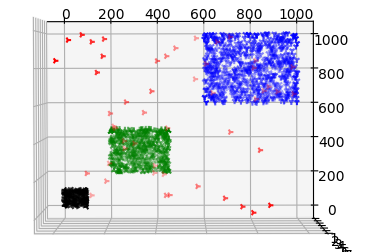
\includegraphics{chap04/LOF_dataset.png}
	\caption{2-D Dataset used for LOF}
\end{figure}

It can be seen from Figure 4.2 that points inside a cluster has LOF values nearly equal to 1 where as noisy points have LOF up to 7. More the LOF score more is the degree of anomaly.

\begin{figure}[h!]
	\centering
	\includegraphics{chap04/LOF_result.png}
	\caption{LOF values for synthetic 2-D dataset}
\end{figure}


\section{MiLOF and MiLOF with RKNN}

We have implemented MiLOF and MiLOF with RKNN in two datasets and measured their efficiency.

\subsection{Performance measures}
Simple accuracy and precision is not the correct measure for these unsupervised anomaly detection problems because the two classes, normal and anomalous are not distributed evenly. So to compare their performance, we compare their false positive rate FPR versus true positive rate TPR.

These performance measures are listed below


\[  Precision \, P = \frac{True Positive }{True Positive + False Positive} \]

 \[  Recall \,  R = \frac{True Positive }{True Positive + False Negative} \]

\[  Flase \, Positive \, Rate \,  (FPR) = \frac{False Positive }{False Positive + True Negative} \]
\\
\\
\subsection{Dataset}
\begin{table}[H]
	\centering
	\caption{Dataset Description}
	\label{my-label}
	\begin{tabular}{|c|c|l|}
		\hline
		\multicolumn{1}{|l|}{} & UCI Letter Dataset & UCI PenDigit Dataset \\ \hline
		n: Data points         & 20000              & 10000                \\ \hline
		d: Dimensions          & 16                 & 16                   \\ \hline
		c: Classes             & 26                 & 10                   \\ \hline
	\end{tabular}
\end{table}



\subsection{Results}

\subsubsection{UCI Letter Dataset}

Following are the reults of different performance measure parameters for both the algorithm by varying K and b(available memory) in UCI letter dataset. 



\begin{table}[H]
	\centering
	\caption{MiLOF and MiLOF with RKNN when K changes while b is kept constant}
	
	\label{my-label}
	\begin{tabular}{|c|c|c|c|c|c|c|c|c|}
		\hline
		\multicolumn{1}{|l|}{}    & \multicolumn{4}{c|}{MiLOF}                                                                                                    & \multicolumn{4}{c|}{MiLOF with RKNN}                                                                                          \\ \hline
		\multicolumn{1}{|l|}{K}   & \multicolumn{1}{l|}{Precision} & \multicolumn{1}{l|}{TPR} & \multicolumn{1}{l|}{FPR} & \multicolumn{1}{l|}{TPR/FPR} & \multicolumn{1}{l|}{Precision} & \multicolumn{1}{l|}{TPR} & \multicolumn{1}{l|}{FPR} & \multicolumn{1}{l|}{TPR/FPR} \\ \hline
		\multicolumn{1}{|l|}{100} & 0.132                          & 0.821                              & 0.1154                   & 7.11                         & 0.348                          & 0.727                              & 0.073                    & 9.945                        \\ \hline
		200                       & 0.12                           & 0.874                              & .146                     & 5.96                         & 0.183                          & 0.704                              & 0.076                    & 9.8                          \\ \hline
		300                       & 0.139                          & 0.84                               & 0.1546                   & 5.441                        & 0.255                          & 0.772                              & 0.069                    & 11.561                       \\ \hline
		400                       & 0.184                          & 0.828                              & 0.140                    & 5.88                         & 0.272                          & 0.804                              & 0.821                    & 9.77                         \\ \hline
		500                       & 0.195                          & 0.781                              & 0.157                    & 4.99                         & 0.305                          & 0.761                              & 0.766                    & 9.70                         \\ \hline
		600                       & 0.229                          & 0.772                              & 0.134                    & 5.536                        & 0.355                          & 0.74                               & 0.072                    & 10.252                       \\ \hline
		700                       & 0.221                          & 0.708                              & 0.141                    & 5.01                         & 0.332                          & 0.591                              & 0.067                    & 8.746                        \\ \hline
	\end{tabular}
\end{table}

\begin{figure}[H]
	\centering
	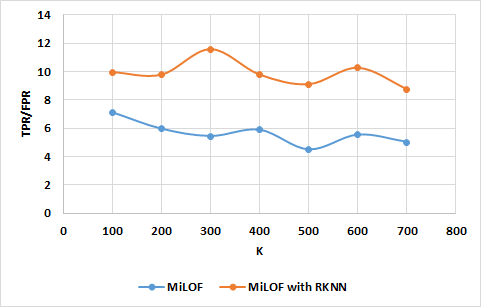
\includegraphics{chap04/varyK.png}
	\caption{TPR/FPR for MiLOF and MiLOF with RKNN when K changes while b is kept constant }
\end{figure}

\begin{table}[H]
	\centering
	\caption{MiLOF and MiLOF with RKNN when b changes while K is kept constant}
	\label{my-label}
	\begin{tabular}{|l|c|c|c|c|c|c|c|c|}
		\hline
		& \multicolumn{4}{c|}{MiLOF}                                                                                                    & \multicolumn{4}{c|}{MiLOF with RKNN}                                                                                          \\ \hline
		b                          & \multicolumn{1}{l|}{Precision} & \multicolumn{1}{l|}{TPR} & \multicolumn{1}{l|}{FPR} & \multicolumn{1}{l|}{TPR/FPR} & \multicolumn{1}{l|}{Precision} & \multicolumn{1}{l|}{TPR} & \multicolumn{1}{l|}{FPR} & \multicolumn{1}{l|}{TPR/FPR} \\ \hline
		2000                       & 0.222                          & 0.707                              & 0.141                    & 5.018                        & 0.332                          & 0.59                               & 0.08                     & 7.35                         \\ \hline
		\multicolumn{1}{|c|}{4000} & 0.291                          & 0.908                              & 0.126                    & 7.215                        & 0.467                          & 0.839                              & 0.054                    & 15.443                       \\ \hline
		\multicolumn{1}{|c|}{5000} & 0.308                          & 0.814                              & 0.103                    & 7.83                         & 0.515                          & 0.856                              & 0.045                    & 18.725                       \\ \hline
		\multicolumn{1}{|c|}{8000} & 0.36                           & 0.915                              & 0.092                    & 9.927                        & 0.67                           & 0.883                              & 0.022                    & 40.89                        \\ \hline
	\end{tabular}
\end{table}


\begin{figure}[H]
	\centering
	\includegraphics{chap04/varyb.png}
	\caption{TPR/FPR for MiLOF and MiLOF with RKNN when b changes while K is constant}
\end{figure}

\subsubsection{UCI Pendigit Dataset}

Following are the reults of different performance measure parameters for both the algorithm by varying K and b(available memory) in UCI pendigit dataset. 

\begin{table}[H]
	\centering
	\caption{MiLOF and MiLOF with RKNN when K changes while b is kept constant}
	\label{my-label}
	\begin{tabular}{|l|c|c|c|c|c|c|c|c|}
		\hline
		& \multicolumn{4}{c|}{MiLOF}                                                                                                    & \multicolumn{4}{c|}{MiLOF with RKNN}                                                                                          \\ \hline
		K                         & \multicolumn{1}{l|}{Precision} & \multicolumn{1}{l|}{TPR} & \multicolumn{1}{l|}{FPR} & \multicolumn{1}{l|}{TPR/FPR} & \multicolumn{1}{l|}{Precision} & \multicolumn{1}{l|}{TPR} & \multicolumn{1}{l|}{FPR} & \multicolumn{1}{l|}{TPR/FPR} \\ \hline
		100                       & 0.618                          & 0.823                              & 0.05                     & 10.98                        & 0.786                          & 0.432                              & 0.0173                   & 24.927                       \\ \hline
		\multicolumn{1}{|c|}{200} & 0.59                           & 0.844                              & 0.099                    & 8.48                         & 0.85                           & 0.463                              & 0.1379                   & 33.569                       \\ \hline
		\multicolumn{1}{|c|}{300} & 0.59                           & 0.783                              & 0.084                    & 9.23                         & 0.773                          & 0.53                               & 0.024                    & 21.748                       \\ \hline
		\multicolumn{1}{|c|}{400} & 0.584                          & 0.7723                             & 0.081                    & 9.455                        & 0.789                          & 0.541                              & 0.0214                   & 25.212                       \\ \hline
		500                       & 0.6203                         & 0.688                              & 0.059                    & 11.628                       & 0.851                          & 0.46                               & 0.011                    & 40.48                        \\ \hline
		600                       & 0.651                          & 0.719                              & 0.045                    & 15.97                        & 0.84                           & 0.67                               & 0.015                    & 44.45                        \\ \hline
		700                       & 0.534                          & 0.739                              & 0.059                    & 12.486                       & 0.797                          & 0.508                              & 0.112                    & 43.65                        \\ \hline
	\end{tabular}
\end{table}



\begin{figure}[H]
	\centering
	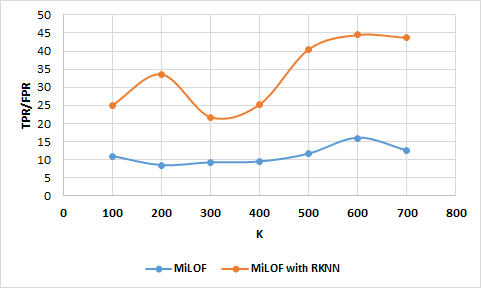
\includegraphics{chap04/varyK2.png}
	\caption{TPR/FPR for MiLOF and MiLOF with RKNN when K changes while b is constant}
\end{figure}



\begin{table}[H]
	\centering
	\caption{MiLOF and MiLOF with RKNN when b changes while K is kept constant}
	\label{my-label}
	\begin{tabular}{|l|c|c|c|c|c|c|c|c|}
		\hline
		& \multicolumn{4}{c|}{MiLOF}                                                                                                    & \multicolumn{4}{c|}{MiLOF with RKNN}                                                                                          \\ \hline
		b                          & \multicolumn{1}{l|}{Precision} & \multicolumn{1}{l|}{TPR} & \multicolumn{1}{l|}{FPR} & \multicolumn{1}{l|}{TPR/FPR} & \multicolumn{1}{l|}{Precision} & \multicolumn{1}{l|}{TPR} & \multicolumn{1}{l|}{FPR} & \multicolumn{1}{l|}{TPR/FPR} \\ \hline
		1000                       & 0.218                          & 0.360                              & .119                     & 3.035                        & 0.1366                         & 0.2158                             & 0.126                    & 1.72                         \\ \hline
		\multicolumn{1}{|c|}{2000} & 0.462                          & 0.412                              & 0.044                    & 9.33                         & 0.471                          & 0.281                              & 0.029                    & 9.678                        \\ \hline
		\multicolumn{1}{|c|}{4000} & 0.5723                         & 0.750                              & 0.052                    & 14.54                        & 0.78                           & 0.65                               & 0.017                    & 38.33                        \\ \hline
		\multicolumn{1}{|c|}{5000} & 0.590                          & 0.794                              & 0.05                     & 15.6                         & 0.79                           & 0.878                              & 0.021                    & 41.22                        \\ \hline
	\end{tabular}
\end{table}

\begin{figure}[H]
	\centering
	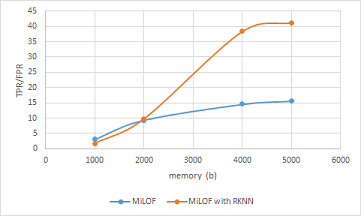
\includegraphics{chap04/varyB2.png}
	\caption{TPR/FPR for MiLOF and MiLOF with RKNN when K changes while b is constant}
\end{figure}
\thispagestyle{empty}
\cleardoublepage


\chapter{Conclusion and Future Scope}\label{Conclusion and Future Scope}
Anomaly detection has many applications in various sectors. However anomaly detection in
streaming data is preferred over static data because its not possible to have and store all the data
in memory. Continuous generation of data and the need to identify the nature of point as fast as
possible motivated us to research on this topic.
Selection of points which are to be summarized and deleted is very crucial because that determines
the accuracy of LOF detection. In MiLOF they select the points which come early in the data stream
assuming that new points are more crucial for anomaly detection. Since there is no selection criteria
for these points many crucial points are summarized and deleted. What we have suggested in MiLOF
with RKNN is that we store number of reverse K nearest neighbors(RKNN) of all the points and
when memory limit is reached we select the points with high RKNN value. High RKNN value here
means the point is surrounded by sufficient number of points which ensures the point to be normal.
By doing so we are keeping the candidate outliers for further computations. From the results plots
it is quite evident that MiLOF with RKNN provides better results then normal MiLOF.

\section{Future Scope}

The outlier detection technique for streaming data discussed in Chapter 3 can be explored further and better summarization techniques other than $c$-means clustering can be used. Deletion of data points with high RKNN values increases the accuracy and hence can be used in many domains like


	\begin{itemize}
		
		\item Fraud detection for credit cards
		\item Intrusion detection
		\item Traffic anomaly detection 
		\item Medical and public health anomaly detection
		\item Sensor networks
	\end{itemize}



\thispagestyle{empty}
\cleardoublepage

\begin{thebibliography}{9}
	
	\bibitem{hawkins}
	 D. M. Hawkins, \textit{Identification of outliers}. Springer, 1980, vol. 11.
	
	\bibitem{a}V. Chandola, A. Banerjee, and V. Kumar, “Anomaly detection: A
	survey,” ACM \textit{Computing Surveys (CSUR)}, vol. 41, no. 3, pp. 1–58, 2009.
	
	\bibitem{b}Markus M. Breunig, Hans-Peter Kriegel, Raymond T. Ng, and Jörg Sander. 2000. LOF: identifying density-based local outliers. SIGMOD Rec. 29, 2 (May 2000), 93-104. 
	
	\bibitem{c}D. Pokrajac, A. Lazarevic, and L. J. Latecki, “Incremental local outlier
	detection for data streams,” in Proc. IEEE Symp. Comput. Intell.
	Data Mining, 2007.
	
	\bibitem{d}M. Salehi, C. Leckie, J. C. Bezdek, T. Vaithianathan and X. Zhang, "Fast Memory Efficient Local Outlier Detection in Data Streams," in IEEE Transactions on Knowledge and Data Engineering, Dec. 1 2016.
	
	\bibitem{e}Fabrizio Angiulli and Fabio Fassetti. 2009. DOLPHIN: An efficient algorithm for mining distance-based outliers in very large datasets. ACM Trans. Knowl.
	
	\bibitem{f}J.Tang, Z. Chen, AW. Fu, D.W. Cheung, Capabilities of outlier detection schemes in large datasets, framework and methodologies Knowledge and Information Systems 11(1), 2006, pp. 45–84.
	
	\bibitem{ca1}
	C. Warrender, S. Forrest, and B. Pearlmutter, “Detecting intrusions using system calls:
	Alternative data models,” in Security and Privacy, 1999. Proceedings of the 1999 IEEE
	Symposium on. IEEE, 1999, pp. 133–145.
	
	\bibitem{ca2}
	C. C. Noble and D. J. Cook, “Graph-based anomaly detection,” in Proceedings of the ninth ACM
	SIGKDD international conference on Knowledge discovery and data mining. ACM, 2003, pp.
	631–636.
	
	\bibitem{ca3}
	S. Shekhar, C.-T. Lu, and P. Zhang, “Detecting graph-based spatial outliers: algorithms and
	applications (a summary of results),” in Proceedings of the seventh ACM SIGKDD international
	conference on Knowledge discovery and data mining. ACM, 2001, pp. 371–376.
	
	\bibitem{contextual}
	X. Song, M. Wu, C. Jermaine, and S. Ranka, “Conditional anomaly detection,” Knowledge and
	Data Engineering, IEEE Transactions on, vol. 19, no. 5, pp. 631–645, 2007.
	
	\bibitem{fraud}
	R. J. Bolton, D. J. Hand et al., “Unsupervised profiling methods for fraud detection,” Credit
	Scoring and Credit Control VII, pp. 235–255, 2001.
	
	\bibitem{medical}
	J. Lin, E. Keogh, A. Fu, and H. Van Herle, “Approximations to magic: Finding unusual medical
	time series,” in Computer-Based Medical Systems, 2005. Proceedings. 18th IEEE Symposium on.
	IEEE, 2005, pp. 329–334.
\end{thebibliography}


\thispagestyle{empty}
\cleardoublepage


%\rhead{\textit{References}}
%\lhead{}
%\renewcommand\bibname{References}

%%%\bibliographystyle{Ref/IEEEtran}
%\bibliographystyle{Ref/asme}
%%%\bibliographystyle{Ref/naturemag}
%%%\bibliographystyle{Ref/bmes}
%%%\bibliographystyle{Ref/achemso}
%%%\bibliographystyle{Ref/rsc}
%%%\bibliographystyle{Ref/osajnl}
%%
%{
%	\fontsize{10}{12}
%	\selectfont
%	\addcontentsline{toc}{chapter}{References}
%	\bibliography{Ref/SampleReferences}
%	\footnotetext{This reference format follows ASME style. You are advised to follow one reference format of any dominant journal of your field.}

%\cleardoublepage
%%% % % % % % % % % % % % % % % % % % % % % % % % % % %
%%% % % % % % % % % % % % % % % % % % % % % % % % % % %

% % % % % % % % % % % % % % % % % % % % % % % % % % %
% % % % % % % % % % % % % % % % % % % % % % % % % % %
\end{document}